\chapter{Steiner Forest algorithms}

\section{Problem description}
Steiner Forest Problem (SFP)\\
Given an undirected graph $G = (V, E)$, a cost function on edges $c : E \rightarrow Q^+$, and a collection of disjoint subsets of $V$, $S_1, \dots S_k$, find a minimum cost subgraph in which each pair of vertices belonging to the same set $S_i$ is connected.
For $k = 1$ the problem is known as Steiner Tree Problem (STP).

\section{Primal-Dual Method algorithm}
Local searches written in our framework were compared to a 2-approximation algorithm described by Vazirani \cite{Vazirani}. As far as we know, it's the best approximation algorithm for a SFP known to date.

The time complexity of provided implementation is $\Oh(S(E + V\alpha(V) + \log(S)))$ where $S = \sum_{i = 1}^{k}S_i$, $\alpha(V)$ is the inverse of the function $n = f(x) = A(x, x)$ and $A$ is Ackermann function.

\section{Create and break cycle local search}
Given some solution to Steiner Forest Problem ,,Create and break cycle'' (CBC) local search changes it by randomly adding edge between solution's vertices. If added edge created a cycle then the heaviest edge from this cycle is removed. It's obvious that obtained graph is still a feasible solution. After described operation it might happen that some edges are no longer needed like for example edges adjacent to leafs that don't belong to $S_i$ for any $i \in \{1, \dots k\}$. Therefore the pruning procedure is used to ensure that only essential edges remain which might lead to further fitness improvement.

Provided Walker implementation takes $\Oh(V\log(V) + KV)$ time to prepare a step, where $K$ is a limit of attempts to choose a random edge with properties as described above. In practice the limit is hardly ever reached and preparing step takes $\Oh(V\log(V)$.

\section{Minimum spanning tree of active vertices local search}
,,MST of active vertices'' (MSTAV) local search starts with some feasible solution of SFP. At each step a new solution is created by computing a pruned minimum spanning tree of $G'$ which is a subgraph of $G$ induced by some set of vertices $V'$ called active vertices. $V'$ is obtained from vertices belonging to the previous solution after randomly applying one of the following operations:
\begin{itemize}
\item add a random vertex that's not already in the set
\item remove a random vertex from the set
\item do both operations described above
\end{itemize}

Note that it might happen that there is no feasible solution in $G'$. Therefore at the end of each step local search checks whether the proposed solution is feasible and if it is not then it reverts any changes.

Provided Walker implementation takes $\Oh(E \log(V))$ time to prepare a step.

\section{Benchmarks}
To compare the algorithms we have used our randomly generated tests and a subset of SteinLib\footnote{\url{http://steinlib.zib.de}} tests for Steiner Tree Problem.
Names of tests generated by us can be expressed as regular expression $[s\ |\ d][E\ |\ R]V<\text{vertices count}>K<\text{terminal vertices count}>$. Letters $s, d$ tells whether the graph is sparse or dense and letters $E, R$ tells accordingly whether the graph is Euclidean or if the edges were given random weight. Descriptions of SteinLib tests can be found at \url{http://steinlib.zib.de}.

In every test Walker starts with a pruned MST as starting solution.
\section{Results}

\subsection{Comparison of hill climbing and simulated annealing convergence}
\FloatBarrier
Experimenting with Walkers utilising StepCtrl that use hill climb and simulated annealing (SA) strategy we have noticed that simulated annealing does not improve fitness of found solutions.
If we consider how presented local searches change depending on StepCtrl we can gain some insight why this happens.
Note that CBC could benefit from SA strategy only when in consecutive iterations chosen edges would create a path leading to cycle creation. There is a little probability of such event especially because the solution is pruned every time edge creating cycle is found. As for MSTAV it allows for adding vertices that might not improve solution immediately even without using simulated annealing strategy therefore introducing this strategy doesn't change much.

\begin{figure}[hb]
\pgfsetplotmarksize{0pt}
\begin{figure}
 \centering
 \caption{\label{CBC-02dEV100K30}CBC-02dEV100K30},
 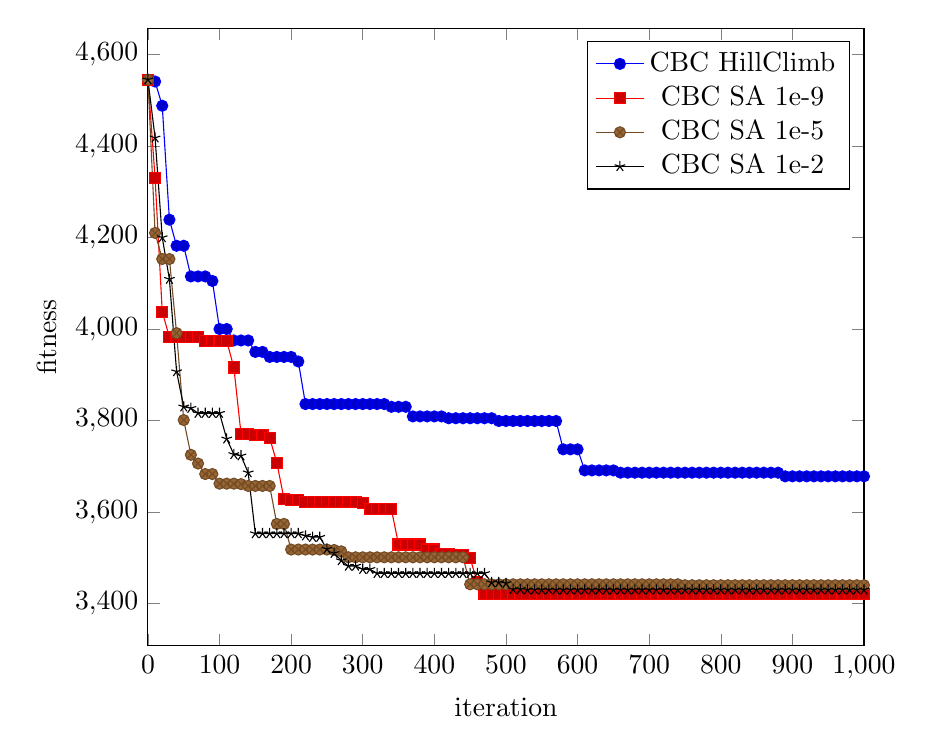
\begin{tikzpicture}
 \begin{axis}[
   width=0.75\textwidth,
   scale only axis,
   xlabel=iteration,
   ylabel=fitness,
   xmin=0,xmax=1000,
   domain=0:1000]
   \addplot coordinates {
     (0,4545)
     (10,4541)
     (20,4488)
     (30,4239)
     (40,4182)
     (50,4182)
     (60,4115)
     (70,4115)
     (80,4115)
     (90,4105)
     (100,4000)
     (110,4000)
     (120,3975)
     (130,3975)
     (140,3975)
     (150,3950)
     (160,3950)
     (170,3939)
     (180,3939)
     (190,3939)
     (200,3939)
     (210,3929)
     (220,3836)
     (230,3836)
     (240,3836)
     (250,3836)
     (260,3836)
     (270,3836)
     (280,3836)
     (290,3836)
     (300,3836)
     (310,3836)
     (320,3836)
     (330,3836)
     (340,3830)
     (350,3830)
     (360,3830)
     (370,3809)
     (380,3809)
     (390,3809)
     (400,3809)
     (410,3809)
     (420,3805)
     (430,3805)
     (440,3805)
     (450,3805)
     (460,3805)
     (470,3805)
     (480,3805)
     (490,3799)
     (500,3799)
     (510,3799)
     (520,3799)
     (530,3799)
     (540,3799)
     (550,3799)
     (560,3799)
     (570,3799)
     (580,3737)
     (590,3737)
     (600,3737)
     (610,3691)
     (620,3691)
     (630,3691)
     (640,3691)
     (650,3691)
     (660,3686)
     (670,3686)
     (680,3686)
     (690,3686)
     (700,3686)
     (710,3686)
     (720,3686)
     (730,3686)
     (740,3686)
     (750,3686)
     (760,3686)
     (770,3686)
     (780,3686)
     (790,3686)
     (800,3686)
     (810,3686)
     (820,3686)
     (830,3686)
     (840,3686)
     (850,3686)
     (860,3686)
     (870,3686)
     (880,3686)
     (890,3678)
     (900,3678)
     (910,3678)
     (920,3678)
     (930,3678)
     (940,3678)
     (950,3678)
     (960,3678)
     (970,3678)
     (980,3678)
     (990,3678)
     (1000,3678)
   };
   \addlegendentry{CBC HillClimb}
   \addplot coordinates {
     (0,4545)
     (10,4330)
     (20,4038)
     (30,3982)
     (40,3982)
     (50,3982)
     (60,3982)
     (70,3982)
     (80,3974)
     (90,3974)
     (100,3974)
     (110,3974)
     (120,3916)
     (130,3771)
     (140,3771)
     (150,3768)
     (160,3768)
     (170,3762)
     (180,3708)
     (190,3629)
     (200,3626)
     (210,3626)
     (220,3621)
     (230,3621)
     (240,3621)
     (250,3621)
     (260,3621)
     (270,3621)
     (280,3621)
     (290,3621)
     (300,3619)
     (310,3606)
     (320,3606)
     (330,3606)
     (340,3606)
     (350,3529)
     (360,3529)
     (370,3529)
     (380,3529)
     (390,3518)
     (400,3518)
     (410,3508)
     (420,3508)
     (430,3506)
     (440,3506)
     (450,3499)
     (460,3446)
     (470,3420)
     (480,3420)
     (490,3420)
     (500,3420)
     (510,3420)
     (520,3420)
     (530,3420)
     (540,3420)
     (550,3420)
     (560,3420)
     (570,3420)
     (580,3420)
     (590,3420)
     (600,3420)
     (610,3420)
     (620,3420)
     (630,3420)
     (640,3420)
     (650,3420)
     (660,3420)
     (670,3420)
     (680,3420)
     (690,3420)
     (700,3420)
     (710,3420)
     (720,3420)
     (730,3420)
     (740,3420)
     (750,3420)
     (760,3420)
     (770,3420)
     (780,3420)
     (790,3420)
     (800,3420)
     (810,3420)
     (820,3420)
     (830,3420)
     (840,3420)
     (850,3420)
     (860,3420)
     (870,3420)
     (880,3420)
     (890,3420)
     (900,3420)
     (910,3420)
     (920,3420)
     (930,3420)
     (940,3420)
     (950,3420)
     (960,3420)
     (970,3420)
     (980,3420)
     (990,3420)
     (1000,3420)
   };
   \addlegendentry{CBC SA 1e-9}
   \addplot coordinates {
     (0,4545)
     (10,4210)
     (20,4153)
     (30,4153)
     (40,3991)
     (50,3801)
     (60,3725)
     (70,3706)
     (80,3683)
     (90,3683)
     (100,3662)
     (110,3662)
     (120,3662)
     (130,3661)
     (140,3657)
     (150,3657)
     (160,3657)
     (170,3657)
     (180,3574)
     (190,3574)
     (200,3518)
     (210,3518)
     (220,3518)
     (230,3518)
     (240,3518)
     (250,3518)
     (260,3517)
     (270,3514)
     (280,3501)
     (290,3501)
     (300,3501)
     (310,3501)
     (320,3501)
     (330,3501)
     (340,3501)
     (350,3501)
     (360,3501)
     (370,3501)
     (380,3501)
     (390,3501)
     (400,3501)
     (410,3501)
     (420,3501)
     (430,3501)
     (440,3501)
     (450,3442)
     (460,3442)
     (470,3442)
     (480,3442)
     (490,3442)
     (500,3442)
     (510,3442)
     (520,3442)
     (530,3442)
     (540,3442)
     (550,3442)
     (560,3442)
     (570,3442)
     (580,3442)
     (590,3442)
     (600,3442)
     (610,3442)
     (620,3442)
     (630,3442)
     (640,3442)
     (650,3442)
     (660,3442)
     (670,3442)
     (680,3442)
     (690,3442)
     (700,3442)
     (710,3442)
     (720,3442)
     (730,3442)
     (740,3442)
     (750,3440)
     (760,3440)
     (770,3440)
     (780,3440)
     (790,3440)
     (800,3440)
     (810,3440)
     (820,3440)
     (830,3440)
     (840,3440)
     (850,3440)
     (860,3440)
     (870,3440)
     (880,3440)
     (890,3440)
     (900,3440)
     (910,3440)
     (920,3440)
     (930,3440)
     (940,3440)
     (950,3440)
     (960,3440)
     (970,3440)
     (980,3440)
     (990,3440)
     (1000,3440)
   };
   \addlegendentry{CBC SA 1e-5}
   \addplot coordinates {
     (0,4545)
     (10,4418)
     (20,4200)
     (30,4109)
     (40,3907)
     (50,3830)
     (60,3827)
     (70,3816)
     (80,3816)
     (90,3816)
     (100,3816)
     (110,3760)
     (120,3726)
     (130,3723)
     (140,3686)
     (150,3553)
     (160,3553)
     (170,3553)
     (180,3553)
     (190,3553)
     (200,3553)
     (210,3553)
     (220,3548)
     (230,3545)
     (240,3545)
     (250,3519)
     (260,3510)
     (270,3494)
     (280,3482)
     (290,3482)
     (300,3475)
     (310,3475)
     (320,3466)
     (330,3466)
     (340,3466)
     (350,3466)
     (360,3466)
     (370,3466)
     (380,3466)
     (390,3466)
     (400,3466)
     (410,3466)
     (420,3466)
     (430,3466)
     (440,3466)
     (450,3466)
     (460,3466)
     (470,3466)
     (480,3446)
     (490,3446)
     (500,3444)
     (510,3431)
     (520,3431)
     (530,3430)
     (540,3430)
     (550,3430)
     (560,3430)
     (570,3430)
     (580,3430)
     (590,3430)
     (600,3430)
     (610,3430)
     (620,3430)
     (630,3430)
     (640,3430)
     (650,3430)
     (660,3430)
     (670,3430)
     (680,3430)
     (690,3430)
     (700,3430)
     (710,3430)
     (720,3430)
     (730,3430)
     (740,3430)
     (750,3430)
     (760,3430)
     (770,3430)
     (780,3430)
     (790,3430)
     (800,3430)
     (810,3430)
     (820,3430)
     (830,3430)
     (840,3430)
     (850,3430)
     (860,3430)
     (870,3430)
     (880,3430)
     (890,3430)
     (900,3430)
     (910,3430)
     (920,3430)
     (930,3430)
     (940,3430)
     (950,3430)
     (960,3430)
     (970,3430)
     (980,3430)
     (990,3430)
     (1000,3430)
   };
   \addlegendentry{CBC SA 1e-2}
 \end{axis}
 \end{tikzpicture}
\end{figure}

\end{figure}
\begin{figure}[hb]
\pgfsetplotmarksize{0pt}
\begin{figure}
 \centering
 \caption{\label{MSTAV-02dEV100K30}MSTAV-02dEV100K30},
 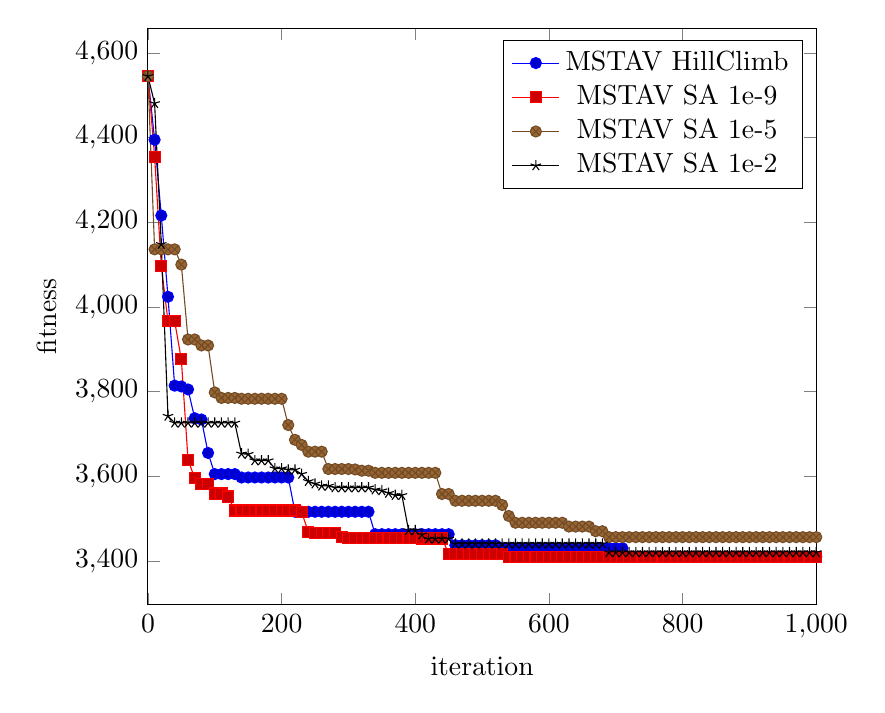
\begin{tikzpicture}
 \begin{axis}[
   width=0.7\textwidth,
   scale only axis,
   xlabel=iteration,
   ylabel=fitness,
   xmin=0,xmax=1000,
   domain=0:1000]
   \addplot coordinates {
     (0,4545)
     (10,4395)
     (20,4216)
     (30,4024)
     (40,3814)
     (50,3812)
     (60,3805)
     (70,3737)
     (80,3734)
     (90,3655)
     (100,3605)
     (110,3605)
     (120,3605)
     (130,3605)
     (140,3597)
     (150,3597)
     (160,3597)
     (170,3597)
     (180,3597)
     (190,3597)
     (200,3597)
     (210,3597)
     (220,3516)
     (230,3516)
     (240,3516)
     (250,3516)
     (260,3516)
     (270,3516)
     (280,3516)
     (290,3516)
     (300,3516)
     (310,3516)
     (320,3516)
     (330,3516)
     (340,3463)
     (350,3463)
     (360,3463)
     (370,3463)
     (380,3463)
     (390,3463)
     (400,3463)
     (410,3463)
     (420,3463)
     (430,3463)
     (440,3463)
     (450,3463)
     (460,3437)
     (470,3437)
     (480,3437)
     (490,3437)
     (500,3437)
     (510,3437)
     (520,3437)
     (530,3430)
     (540,3430)
     (550,3430)
     (560,3430)
     (570,3430)
     (580,3430)
     (590,3430)
     (600,3430)
     (610,3430)
     (620,3430)
     (630,3430)
     (640,3430)
     (650,3430)
     (660,3430)
     (670,3430)
     (680,3430)
     (690,3430)
     (700,3430)
     (710,3430)
     (720,3410)
     (730,3410)
     (740,3410)
     (750,3410)
     (760,3410)
     (770,3410)
     (780,3410)
     (790,3410)
     (800,3410)
     (810,3410)
     (820,3410)
     (830,3410)
     (840,3410)
     (850,3410)
     (860,3410)
     (870,3410)
     (880,3410)
     (890,3410)
     (900,3410)
     (910,3410)
     (920,3410)
     (930,3410)
     (940,3410)
     (950,3410)
     (960,3410)
     (970,3410)
     (980,3410)
     (990,3410)
     (1000,3410)
   };
   \addlegendentry{MSTAV HillClimb}
   \addplot coordinates {
     (0,4545)
     (10,4355)
     (20,4097)
     (30,3966)
     (40,3966)
     (50,3876)
     (60,3639)
     (70,3595)
     (80,3581)
     (90,3581)
     (100,3559)
     (110,3559)
     (120,3552)
     (130,3519)
     (140,3519)
     (150,3519)
     (160,3519)
     (170,3519)
     (180,3519)
     (190,3519)
     (200,3519)
     (210,3519)
     (220,3519)
     (230,3515)
     (240,3468)
     (250,3465)
     (260,3465)
     (270,3465)
     (280,3465)
     (290,3457)
     (300,3454)
     (310,3454)
     (320,3454)
     (330,3454)
     (340,3454)
     (350,3454)
     (360,3454)
     (370,3454)
     (380,3454)
     (390,3454)
     (400,3454)
     (410,3453)
     (420,3453)
     (430,3453)
     (440,3453)
     (450,3417)
     (460,3417)
     (470,3417)
     (480,3417)
     (490,3417)
     (500,3417)
     (510,3417)
     (520,3417)
     (530,3417)
     (540,3410)
     (550,3410)
     (560,3410)
     (570,3410)
     (580,3410)
     (590,3410)
     (600,3410)
     (610,3410)
     (620,3410)
     (630,3410)
     (640,3410)
     (650,3410)
     (660,3410)
     (670,3410)
     (680,3410)
     (690,3410)
     (700,3410)
     (710,3410)
     (720,3410)
     (730,3410)
     (740,3410)
     (750,3410)
     (760,3410)
     (770,3410)
     (780,3410)
     (790,3410)
     (800,3410)
     (810,3410)
     (820,3410)
     (830,3410)
     (840,3410)
     (850,3410)
     (860,3410)
     (870,3410)
     (880,3410)
     (890,3410)
     (900,3410)
     (910,3410)
     (920,3410)
     (930,3410)
     (940,3410)
     (950,3410)
     (960,3410)
     (970,3410)
     (980,3410)
     (990,3410)
     (1000,3410)
   };
   \addlegendentry{MSTAV SA 1e-9}
   \addplot coordinates {
     (0,4545)
     (10,4136)
     (20,4136)
     (30,4136)
     (40,4136)
     (50,4100)
     (60,3923)
     (70,3923)
     (80,3909)
     (90,3909)
     (100,3798)
     (110,3785)
     (120,3785)
     (130,3785)
     (140,3783)
     (150,3783)
     (160,3783)
     (170,3783)
     (180,3783)
     (190,3783)
     (200,3783)
     (210,3721)
     (220,3686)
     (230,3674)
     (240,3658)
     (250,3658)
     (260,3658)
     (270,3617)
     (280,3617)
     (290,3617)
     (300,3617)
     (310,3616)
     (320,3613)
     (330,3613)
     (340,3608)
     (350,3608)
     (360,3608)
     (370,3608)
     (380,3608)
     (390,3608)
     (400,3608)
     (410,3608)
     (420,3608)
     (430,3608)
     (440,3558)
     (450,3558)
     (460,3542)
     (470,3542)
     (480,3542)
     (490,3542)
     (500,3542)
     (510,3542)
     (520,3542)
     (530,3532)
     (540,3506)
     (550,3490)
     (560,3490)
     (570,3490)
     (580,3490)
     (590,3490)
     (600,3490)
     (610,3490)
     (620,3490)
     (630,3481)
     (640,3481)
     (650,3481)
     (660,3481)
     (670,3470)
     (680,3470)
     (690,3456)
     (700,3456)
     (710,3456)
     (720,3456)
     (730,3456)
     (740,3456)
     (750,3456)
     (760,3456)
     (770,3456)
     (780,3456)
     (790,3456)
     (800,3456)
     (810,3456)
     (820,3456)
     (830,3456)
     (840,3456)
     (850,3456)
     (860,3456)
     (870,3456)
     (880,3456)
     (890,3456)
     (900,3456)
     (910,3456)
     (920,3456)
     (930,3456)
     (940,3456)
     (950,3456)
     (960,3456)
     (970,3456)
     (980,3456)
     (990,3456)
     (1000,3456)
   };
   \addlegendentry{MSTAV SA 1e-5}
   \addplot coordinates {
     (0,4545)
     (10,4481)
     (20,4148)
     (30,3742)
     (40,3726)
     (50,3726)
     (60,3726)
     (70,3726)
     (80,3726)
     (90,3726)
     (100,3726)
     (110,3726)
     (120,3726)
     (130,3726)
     (140,3653)
     (150,3652)
     (160,3637)
     (170,3637)
     (180,3637)
     (190,3618)
     (200,3618)
     (210,3615)
     (220,3615)
     (230,3605)
     (240,3588)
     (250,3582)
     (260,3577)
     (270,3577)
     (280,3573)
     (290,3573)
     (300,3573)
     (310,3573)
     (320,3573)
     (330,3573)
     (340,3568)
     (350,3566)
     (360,3560)
     (370,3555)
     (380,3555)
     (390,3472)
     (400,3472)
     (410,3462)
     (420,3452)
     (430,3452)
     (440,3452)
     (450,3452)
     (460,3440)
     (470,3440)
     (480,3440)
     (490,3440)
     (500,3440)
     (510,3440)
     (520,3440)
     (530,3440)
     (540,3440)
     (550,3440)
     (560,3440)
     (570,3440)
     (580,3440)
     (590,3440)
     (600,3440)
     (610,3440)
     (620,3440)
     (630,3440)
     (640,3440)
     (650,3440)
     (660,3440)
     (670,3440)
     (680,3440)
     (690,3420)
     (700,3420)
     (710,3420)
     (720,3420)
     (730,3420)
     (740,3420)
     (750,3420)
     (760,3420)
     (770,3420)
     (780,3420)
     (790,3420)
     (800,3420)
     (810,3420)
     (820,3420)
     (830,3420)
     (840,3420)
     (850,3420)
     (860,3420)
     (870,3420)
     (880,3420)
     (890,3420)
     (900,3420)
     (910,3420)
     (920,3420)
     (930,3420)
     (940,3420)
     (950,3420)
     (960,3420)
     (970,3420)
     (980,3420)
     (990,3420)
     (1000,3420)
   };
   \addlegendentry{MSTAV SA 1e-2}
 \end{axis}
 \end{tikzpicture}
\end{figure}

\end{figure}
\FloatBarrier

\subsection{CBC's and MSTAV's search space topology comparison}
\FloatBarrier
Benchmarks have shown that MSTAV local search performs definitely better than CBC. If we take a closer look at each algorithm's search space topology we might find what is the cause. What seems to be the key difference in MSTAV's and CBC's search space topology is the existence of plateau areas. MSTAV's might add additional vertex to set of active vertices while keeping the same fitness because the pruned MST that is computed during each step may not include newly added vertex. On the other hand CBC with StepCtrl using hill climbing strategy makes step only if it finds strictly better solution. If we combine that with observation that only edges between vertices of current solution allows to create a cycle in a single step we can notice that solution's neighbourhood is pretty small and steep. Which might be the reason why CBC gets stuck in local optima more often than MSTAV.
\begin{figure}[hb]
\pgfsetplotmarksize{0pt}
\begin{figure}
 \centering
 \caption{\label{CBCvsMSTAV-d05}CBCvsMSTAV-d05},
 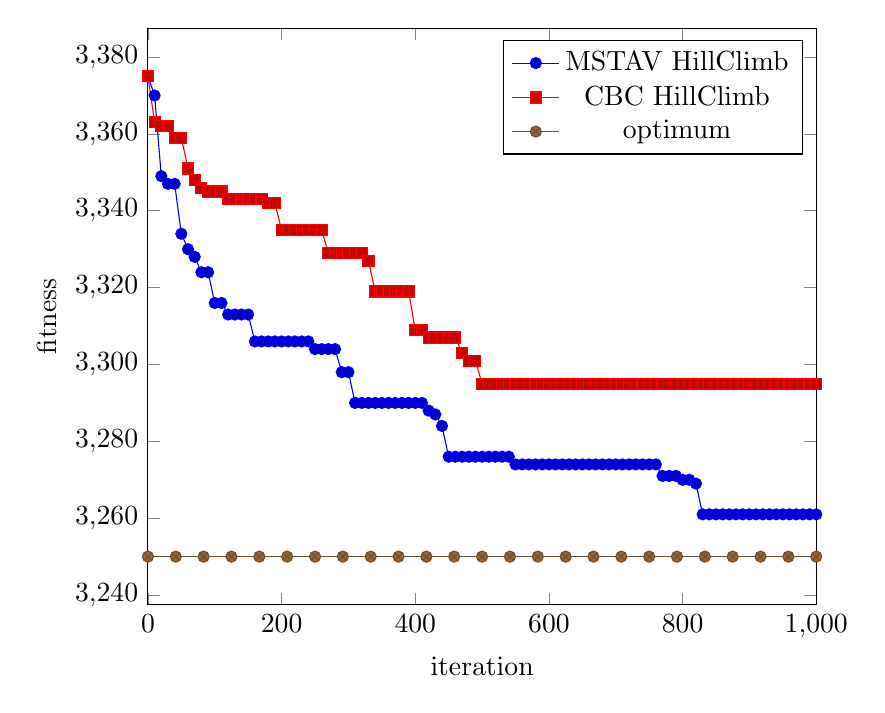
\begin{tikzpicture}
 \begin{axis}[
   width=0.7\textwidth,
   scale only axis,
   xlabel=iteration,
   ylabel=fitness,
   xmin=0,xmax=1000,
   domain=0:1000]
   \addplot coordinates {
     (0,3375)
     (10,3370)
     (20,3349)
     (30,3347)
     (40,3347)
     (50,3334)
     (60,3330)
     (70,3328)
     (80,3324)
     (90,3324)
     (100,3316)
     (110,3316)
     (120,3313)
     (130,3313)
     (140,3313)
     (150,3313)
     (160,3306)
     (170,3306)
     (180,3306)
     (190,3306)
     (200,3306)
     (210,3306)
     (220,3306)
     (230,3306)
     (240,3306)
     (250,3304)
     (260,3304)
     (270,3304)
     (280,3304)
     (290,3298)
     (300,3298)
     (310,3290)
     (320,3290)
     (330,3290)
     (340,3290)
     (350,3290)
     (360,3290)
     (370,3290)
     (380,3290)
     (390,3290)
     (400,3290)
     (410,3290)
     (420,3288)
     (430,3287)
     (440,3284)
     (450,3276)
     (460,3276)
     (470,3276)
     (480,3276)
     (490,3276)
     (500,3276)
     (510,3276)
     (520,3276)
     (530,3276)
     (540,3276)
     (550,3274)
     (560,3274)
     (570,3274)
     (580,3274)
     (590,3274)
     (600,3274)
     (610,3274)
     (620,3274)
     (630,3274)
     (640,3274)
     (650,3274)
     (660,3274)
     (670,3274)
     (680,3274)
     (690,3274)
     (700,3274)
     (710,3274)
     (720,3274)
     (730,3274)
     (740,3274)
     (750,3274)
     (760,3274)
     (770,3271)
     (780,3271)
     (790,3271)
     (800,3270)
     (810,3270)
     (820,3269)
     (830,3261)
     (840,3261)
     (850,3261)
     (860,3261)
     (870,3261)
     (880,3261)
     (890,3261)
     (900,3261)
     (910,3261)
     (920,3261)
     (930,3261)
     (940,3261)
     (950,3261)
     (960,3261)
     (970,3261)
     (980,3261)
     (990,3261)
     (1000,3261)
   };
   \addlegendentry{MSTAV HillClimb}
   \addplot coordinates {
     (0,3375)
     (10,3363)
     (20,3362)
     (30,3362)
     (40,3359)
     (50,3359)
     (60,3351)
     (70,3348)
     (80,3346)
     (90,3345)
     (100,3345)
     (110,3345)
     (120,3343)
     (130,3343)
     (140,3343)
     (150,3343)
     (160,3343)
     (170,3343)
     (180,3342)
     (190,3342)
     (200,3335)
     (210,3335)
     (220,3335)
     (230,3335)
     (240,3335)
     (250,3335)
     (260,3335)
     (270,3329)
     (280,3329)
     (290,3329)
     (300,3329)
     (310,3329)
     (320,3329)
     (330,3327)
     (340,3319)
     (350,3319)
     (360,3319)
     (370,3319)
     (380,3319)
     (390,3319)
     (400,3309)
     (410,3309)
     (420,3307)
     (430,3307)
     (440,3307)
     (450,3307)
     (460,3307)
     (470,3303)
     (480,3301)
     (490,3301)
     (500,3295)
     (510,3295)
     (520,3295)
     (530,3295)
     (540,3295)
     (550,3295)
     (560,3295)
     (570,3295)
     (580,3295)
     (590,3295)
     (600,3295)
     (610,3295)
     (620,3295)
     (630,3295)
     (640,3295)
     (650,3295)
     (660,3295)
     (670,3295)
     (680,3295)
     (690,3295)
     (700,3295)
     (710,3295)
     (720,3295)
     (730,3295)
     (740,3295)
     (750,3295)
     (760,3295)
     (770,3295)
     (780,3295)
     (790,3295)
     (800,3295)
     (810,3295)
     (820,3295)
     (830,3295)
     (840,3295)
     (850,3295)
     (860,3295)
     (870,3295)
     (880,3295)
     (890,3295)
     (900,3295)
     (910,3295)
     (920,3295)
     (930,3295)
     (940,3295)
     (950,3295)
     (960,3295)
     (970,3295)
     (980,3295)
     (990,3295)
     (1000,3295)
   };
   \addlegendentry{CBC HillClimb}
   \addplot {3250.000000};
   \addlegendentry{optimum}
 \end{axis}
 \end{tikzpicture}
\end{figure}

\end{figure}
\FloatBarrier

\subsection{Comparison of found solutions' fitness}
\FloatBarrier
After testing presented algorithms we have made the following observations:
\begin{itemize}
\item fitness of solutions found by 2-approximation algorithm is almost always less than 1.1 times optimum
\item local searches performed well on problem instances with less than thousand of vertices
\item MSTAV gives better results than CBC most of the time
\item MSTAV often finds better solutions than 2-approximation algorithm for problem instances with less than thousand of vertices
\item for graphs with thousands of vertices 2-approximation algorithm finds much better solutions than local searches
\end{itemize}

\begin{figure}[hb]
  \centering
  \begin{tabular}[ht]{|l||c|c|c|c|H}
\cline{1-5}
 & 01dEV100K20 & 01sEV1000K150 & 01sEV100K20 & 01dRV100K20 & \\ \cline{1-5}\cline{1-5} 
2-Approximation &3476 & 20605 & 5927 & 24 & \\ \cline{1-5}
MSTAV HillClimb &3376 & 20231 & 5785 & 22 & \\ \cline{1-5}
CBC HillClimb &3654 & 24213 & 6021 & 24 & \\ \cline{1-5}
\end{tabular}
  \caption{Results for sample of SFP tests for graphs with less than thousand vertices}
\end{figure}

\begin{figure}[hb]
  \centering
  \begin{tabular}[ht]{|l||c|c|c|c|c|c|H}
\cline{1-7}
 & alut2764 & b13 & berlin52 & diw0250 & msm3277 & d15 & \\ \cline{1-7}\cline{1-7} 
Optimum &640 & 165 & 1044 & 350 & 869 & 1116 & \\ \cline{1-7}
2-Approximation &710 & 187 & 1078 & 363 & 912 & 1161 & \\ \cline{1-7}
MSTAV HillClimb &662 & 170 & 1044 & 467 & 1089 & 1126 & \\ \cline{1-7}
CBC HillClimb &1044 & 177 & 1103 & 518 & 1222 & 1186 & \\ \cline{1-7}
\end{tabular}
  \caption{Results for sample of STP tests for graphs with less than thousand vertices}
\end{figure}

\begin{figure}[hb]
  \centering
  \begin{tabular}[ht]{|l||c|c|c|c|H}
\cline{1-5}
 & 04sEV1000K250 & 03sEV1000K150 & 01sRV1000K150 & 01sRV1000K250 & \\ \cline{1-5}\cline{1-5} 
2-Approximation &29569 & 17175 & 208 & 262 & \\ \cline{1-5}
MSTAV HillClimb &29624 & 17163 & 196 & 279 & \\ \cline{1-5}
CBC HillClimb &35091 & 21899 & 259 & 365 & \\ \cline{1-5}
\end{tabular}
  \caption{Results for sample of SFP tests for graphs with at least thousand of vertices}
\end{figure}

\begin{figure}[hb]
  \centering
  \begin{tabular}[ht]{|l||c|c|c|c|c|c|H}
\cline{1-7}
 & alue2087 & d11 & diw0445 & e02 & taq0431 & msm3277 & \\ \cline{1-7}\cline{1-7} 
Optimum &1049 & 29 & 1363 & 214 & 897 & 869 & \\ \cline{1-7}
2-Approximation &1122 & 33 & 1453 & 255 & 980 & 912 & \\ \cline{1-7}
MSTAV HillClimb &1375 & 36 & 1827 & 361 & 1484 & 1233 & \\ \cline{1-7}
CBC HillClimb &1698 & 49 & 2321 & 442 & 1519 & 1263 & \\ \cline{1-7}
\end{tabular}
  \caption{Results for sample of STP tests for graphs with at least thousand of vertices}
\end{figure}

\FloatBarrier
